\documentclass[8pt,aspectratio=169]{beamer}
\usetheme{Madrid}
\usepackage{graphicx}
\usepackage{booktabs}
\usepackage{adjustbox}
\usepackage{multicol}
\usepackage{amsmath}
\usepackage{listings}
\usepackage{xcolor}

% Color definitions
\definecolor{mlblue}{RGB}{0,102,204}
\definecolor{mlpurple}{RGB}{51,51,178}
\definecolor{mllavender}{RGB}{173,173,224}
\definecolor{mllavender2}{RGB}{193,193,232}
\definecolor{mllavender3}{RGB}{204,204,235}
\definecolor{mllavender4}{RGB}{214,214,239}
\definecolor{mlorange}{RGB}{255, 127, 14}
\definecolor{mlgreen}{RGB}{44, 160, 44}
\definecolor{mlred}{RGB}{214, 39, 40}
\definecolor{mlgray}{RGB}{127, 127, 127}

% Additional colors for template compatibility
\definecolor{lightgray}{RGB}{240, 240, 240}
\definecolor{midgray}{RGB}{180, 180, 180}

% Apply custom colors to Madrid theme
\setbeamercolor{palette primary}{bg=mllavender3,fg=mlpurple}
\setbeamercolor{palette secondary}{bg=mllavender2,fg=mlpurple}
\setbeamercolor{palette tertiary}{bg=mllavender,fg=white}
\setbeamercolor{palette quaternary}{bg=mlpurple,fg=white}

\setbeamercolor{structure}{fg=mlpurple}
\setbeamercolor{section in toc}{fg=mlpurple}
\setbeamercolor{subsection in toc}{fg=mlblue}
\setbeamercolor{title}{fg=mlpurple}
\setbeamercolor{frametitle}{fg=mlpurple,bg=mllavender3}
\setbeamercolor{block title}{bg=mllavender2,fg=mlpurple}
\setbeamercolor{block body}{bg=mllavender4,fg=black}

% Remove navigation symbols
\setbeamertemplate{navigation symbols}{}

% Clean itemize/enumerate
\setbeamertemplate{itemize items}[circle]
\setbeamertemplate{enumerate items}[default]

% Reduce margins for more content space
\setbeamersize{text margin left=5mm,text margin right=5mm}

% Command for bottom annotation (Madrid-style)
\newcommand{\bottomnote}[1]{%
\vfill
\vspace{-2mm}
\textcolor{mllavender2}{\rule{\textwidth}{0.4pt}}
\vspace{1mm}
\footnotesize
\textbf{#1}
}

% TikZ and pgfplots packages
\usepackage{tikz}
\usepackage{pgfplots}
\pgfplotsset{compat=1.18}
\usetikzlibrary{arrows.meta, positioning, shapes.geometric, shapes.symbols, calc, decorations.pathmorphing}

% Silence benign pgfkeys warning about /tikz/step from beamer enumerate style
\pgfplotsset{
  every axis/.append style={
    /pgf/number format/1000 sep={}
  }
}

\title{Cryptography \& Security: Course Preview}
\subtitle{INTRO Preview -- What You Will Learn}
\author{Prof.~Dr.~Joerg Osterrieder}
\institute{University Lecture Series}
\date{\today}

\begin{document}

%--- Frame 1: Title ---
\begin{frame}
  \titlepage
\end{frame}

%--- Frame 2: Hash Function Anatomy ---
\begin{frame}{Hash Function Anatomy}
\begin{center}
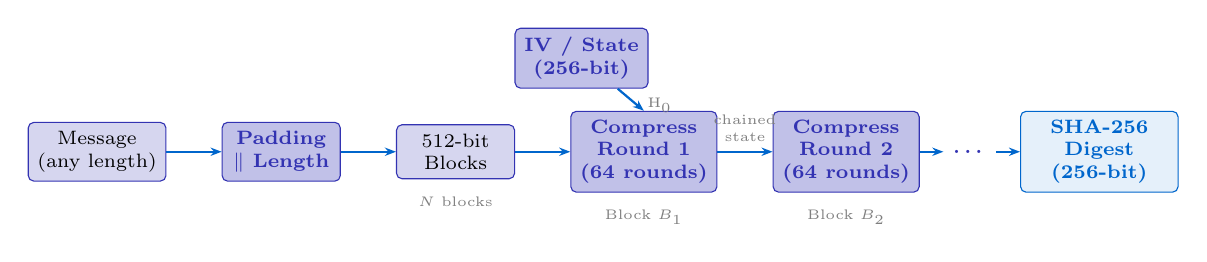
\begin{tikzpicture}[
  node distance=0.55cm and 0.7cm,
  box/.style={rectangle, rounded corners=2pt, draw=mlpurple, fill=mllavender4,
              minimum width=1.5cm, minimum height=0.55cm, font=\scriptsize, align=center},
  opbox/.style={rectangle, rounded corners=2pt, draw=mlpurple, fill=mllavender2,
                minimum width=1.5cm, minimum height=0.55cm, font=\scriptsize\bfseries, align=center, text=mlpurple},
  outbox/.style={rectangle, rounded corners=2pt, draw=mlblue, fill=mlblue!10,
                 minimum width=2.0cm, minimum height=0.55cm, font=\scriptsize\bfseries, align=center, text=mlblue},
  arr/.style={-{Stealth[length=4pt]}, thick, color=mlblue},
  lbl/.style={font=\tiny, color=mlgray}
]
  % Input
  \node[box] (msg) {Message\\(any length)};
  % Padding
  \node[opbox, right=of msg] (pad) {Padding\\$\|$ Length};
  % Padded block label
  \node[box, right=of pad] (split) {512-bit\\Blocks};
  % IV node above compression
  \node[opbox, above=0.45cm of split, xshift=1.6cm] (iv) {IV / State\\(256-bit)};
  % Compression rounds
  \node[opbox, right=of split] (comp1) {Compress\\Round 1\\(64 rounds)};
  \node[opbox, right=of comp1] (comp2) {Compress\\Round 2\\(64 rounds)};
  % Dots
  \node[font=\scriptsize\bfseries, right=0.3cm of comp2, color=mlpurple] (dots) {\ldots};
  % Digest output
  \node[outbox, right=0.3cm of dots] (digest) {SHA-256\\Digest\\(256-bit)};

  % Arrows
  \draw[arr] (msg) -- (pad);
  \draw[arr] (pad) -- (split);
  \draw[arr] (split) -- (comp1);
  \draw[arr] (comp1) -- (comp2) node[midway, above, lbl, align=center] {chained\\state};
  \draw[arr] (comp2) -- (dots);
  \draw[arr] (dots) -- (digest);
  \draw[arr] (iv) -- (comp1.north) node[near end, right, lbl] {H$_0$};
  % Feedback arrow comp1->comp2 already covered; add chain label comp2->dots
  % Block labels below
  \node[lbl, below=0.1cm of split] {$N$ blocks};
  \node[lbl, below=0.1cm of comp1] {Block $B_1$};
  \node[lbl, below=0.1cm of comp2] {Block $B_2$};
\end{tikzpicture}
\end{center}
\vspace{-1mm}
\begin{columns}[T]
  \column{0.33\textwidth}
    \textbf{\textcolor{mlpurple}{Input Processing}}\\
    \scriptsize Append bit \texttt{1}, pad to $\equiv 448 \pmod{512}$, append 64-bit length.
  \column{0.34\textwidth}
    \textbf{\textcolor{mlpurple}{Compression Function}}\\
    \scriptsize 64 rounds per block; eight 32-bit state words ($a$--$h$); Ch, Maj, $\Sigma$ operations.
  \column{0.33\textwidth}
    \textbf{\textcolor{mlblue}{Output}}\\
    \scriptsize 256-bit digest; collision resistance $\approx 2^{128}$; pre-image resistance $\approx 2^{256}$.
\end{columns}
\bottomnote{SHA-256 (FIPS 180-4) -- Merkle-Damg\r{a}rd construction -- 512-bit blocks, 64 rounds, 256-bit state}
\end{frame}

%--- Frame 3: ECDSA Signature Flow ---
\begin{frame}{ECDSA Signature Flow}
\begin{columns}[T]
\column{0.62\textwidth}
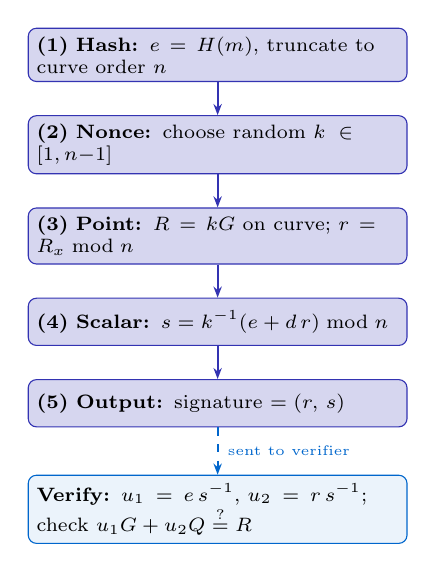
\begin{tikzpicture}[
  node distance=0.42cm and 1.1cm,
  procstep/.style={rectangle, rounded corners=3pt, draw=mlpurple, fill=mllavender4,
               minimum width=4.8cm, minimum height=0.6cm, font=\scriptsize, align=left,
               text width=4.6cm, inner sep=3pt},
  vprocstep/.style={rectangle, rounded corners=3pt, draw=mlblue, fill=mlblue!8,
                minimum width=4.8cm, minimum height=0.6cm, font=\scriptsize, align=left,
                text width=4.6cm, inner sep=3pt},
  arr/.style={-{Stealth[length=4pt]}, thick, color=mlpurple},
  lbl/.style={font=\tiny\bfseries, color=mlpurple, left=1pt}
]
  \node[procstep] (s1) {\textbf{(1) Hash:} $e = H(m)$, truncate to curve order $n$};
  \node[procstep, below=of s1] (s2) {\textbf{(2) Nonce:} choose random $k \in [1,n{-}1]$};
  \node[procstep, below=of s2] (s3) {\textbf{(3) Point:} $R = kG$ on curve; $r = R_x \bmod n$};
  \node[procstep, below=of s3] (s4) {\textbf{(4) Scalar:} $s = k^{-1}(e + d\,r) \bmod n$};
  \node[procstep, below=of s4] (s5) {\textbf{(5) Output:} signature $= (r,\,s)$};
  \node[vprocstep, below=0.6cm of s5] (v1)
    {\textbf{Verify:} $u_1 = e\,s^{-1}$,\ $u_2 = r\,s^{-1}$;\ check $u_1 G + u_2 Q \stackrel{?}{=} R$};

  \draw[arr] (s1) -- (s2);
  \draw[arr] (s2) -- (s3);
  \draw[arr] (s3) -- (s4);
  \draw[arr] (s4) -- (s5);
  \draw[-{Stealth[length=4pt]}, thick, color=mlblue, dashed] (s5) -- (v1)
    node[midway, right, font=\tiny, color=mlblue] {sent to verifier};
\end{tikzpicture}

\column{0.38\textwidth}
\vspace{2mm}
\textbf{\textcolor{mlpurple}{Key Variables}}\\[2pt]
\scriptsize
\begin{tabular}{@{}ll@{}}
$G$ & base point on curve \\
$n$ & curve order \\
$d$ & private key (scalar) \\
$Q = dG$ & public key (point) \\
$k$ & ephemeral nonce \\
$r, s$ & signature components \\
\end{tabular}

\vspace{4mm}
\textbf{\textcolor{mlred}{Security Note}}\\[2pt]
\scriptsize Never reuse $k$! Same $k$ for two different messages exposes private key $d$.\\[4pt]
\textbf{\textcolor{mlblue}{Curve Parameters}}\\[2pt]
\scriptsize secp256k1 (Bitcoin):\\256-bit field, $\approx 2^{128}$ security.
\end{columns}
\bottomnote{ECDSA (ANSI X9.62) -- secp256k1 used in Bitcoin/Ethereum -- Nonce reuse is catastrophic}
\end{frame}

%--- Frame 4: Key Sizes vs Security Levels ---
\begin{frame}{Key Sizes vs.\ Security Levels}
\begin{center}
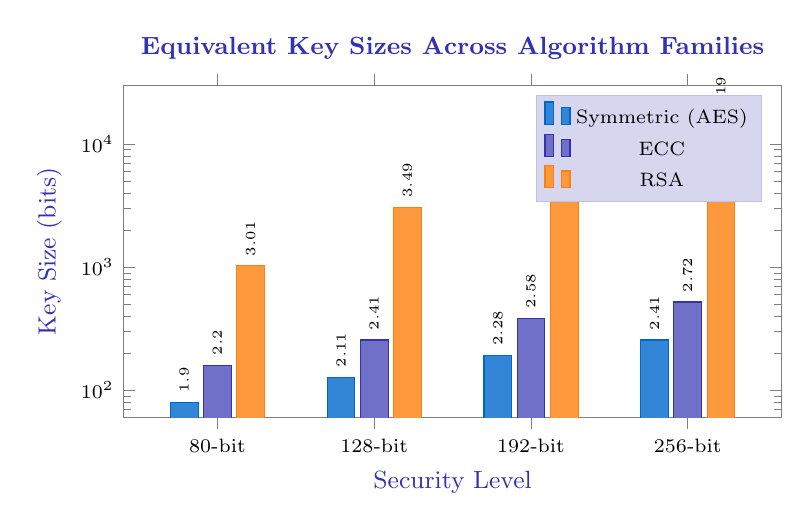
\begin{tikzpicture}
\begin{axis}[
  width=0.82\textwidth, height=5.8cm,
  ybar, bar width=10pt,
  ymode=log, log basis y=10,
  ymin=60, ymax=30000,
  xtick={1,2,3,4},
  xticklabels={80-bit,128-bit,192-bit,256-bit},
  xlabel={\small Security Level},
  ylabel={\small Key Size (bits)},
  xlabel style={color=mlpurple, font=\small},
  ylabel style={color=mlpurple, font=\small},
  tick label style={font=\scriptsize},
  legend style={at={(0.97,0.97)}, anchor=north east, font=\scriptsize,
                draw=mllavender2, fill=mllavender4},
  title style={font=\small\bfseries, color=mlpurple},
  title={Equivalent Key Sizes Across Algorithm Families},
  enlarge x limits=0.2,
  nodes near coords,
  nodes near coords style={font=\tiny, rotate=90, anchor=west, color=black},
  every axis plot/.append style={draw=none},
  axis line style={color=mlgray},
  tick style={color=mlgray},
]
  % Symmetric (AES)
  \addplot[fill=mlblue!80, draw=mlblue] coordinates {(1,80) (2,128) (3,192) (4,256)};
  % ECC
  \addplot[fill=mlpurple!70, draw=mlpurple] coordinates {(1,160) (2,256) (3,384) (4,521)};
  % RSA
  \addplot[fill=mlorange!80, draw=mlorange] coordinates {(1,1024) (2,3072) (3,7680) (4,15360)};
  \legend{Symmetric (AES), ECC, RSA}
\end{axis}
\end{tikzpicture}
\end{center}
\bottomnote{NIST SP 800-57 -- RSA key sizes grow exponentially; ECC provides equivalent security with far smaller keys}
\end{frame}

%--- Frame 5: Algorithm Performance Comparison ---
\begin{frame}{Algorithm Performance Comparison}
\begin{center}
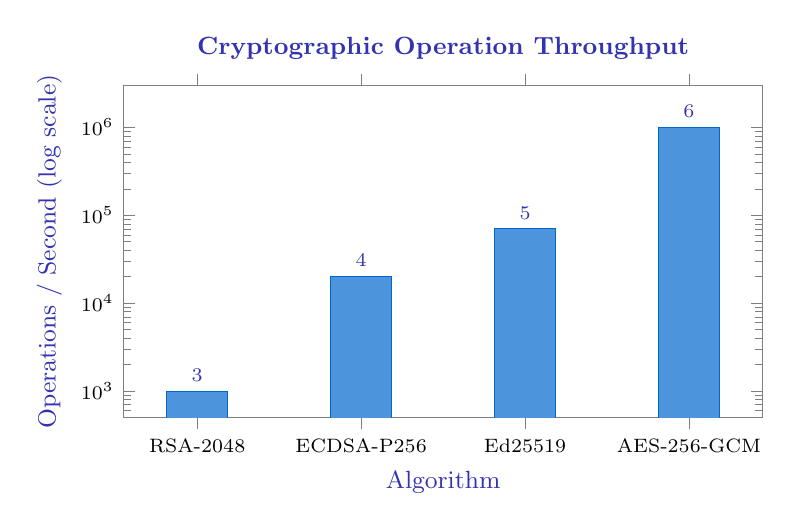
\begin{tikzpicture}
\begin{axis}[
  width=0.80\textwidth, height=5.8cm,
  ybar, bar width=22pt,
  ymode=log, log basis y=10,
  ymin=500, ymax=3000000,
  symbolic x coords={RSA-2048, ECDSA-P256, Ed25519, AES-256-GCM},
  xtick=data,
  xlabel={\small Algorithm},
  ylabel={\small Operations / Second (log scale)},
  xlabel style={color=mlpurple, font=\small},
  ylabel style={color=mlpurple, font=\small},
  tick label style={font=\scriptsize},
  title={Cryptographic Operation Throughput},
  title style={font=\small\bfseries, color=mlpurple},
  nodes near coords,
  nodes near coords style={font=\scriptsize\bfseries, anchor=south, color=mlpurple},
  every node near coord/.append style={/pgf/number format/fixed, /pgf/number format/precision=0},
  enlarge x limits=0.15,
  axis line style={color=mlgray},
  tick style={color=mlgray},
]
  \addplot[fill=mlblue!70, draw=mlblue] coordinates {
    (RSA-2048,   1000)
    (ECDSA-P256, 20000)
    (Ed25519,    70000)
    (AES-256-GCM,1000000)
  };
\end{axis}
\end{tikzpicture}
\end{center}
\vspace{-2mm}
\scriptsize
\textcolor{mlpurple}{\textbf{Key takeaway:}} AES-256-GCM (symmetric) is $\sim$1000$\times$ faster than RSA-2048. Ed25519 outperforms ECDSA-P256 by $3.5\times$ with equivalent security. Use hybrid encryption in practice.
\bottomnote{Indicative benchmarks on modern x86-64 hardware -- actual throughput varies by implementation and hardware acceleration}
\end{frame}

%--- Frame 6: Crypto Adoption Timeline ---
\begin{frame}{Crypto Adoption Timeline (2010--2025)}
\begin{center}
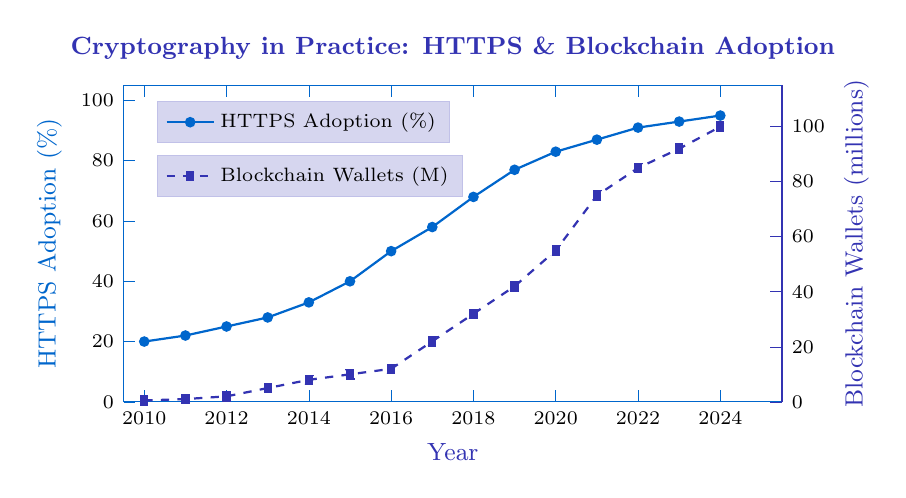
\begin{tikzpicture}
\pgfplotsset{set layers}
\begin{axis}[
  name=ax1,
  width=0.82\textwidth, height=5.6cm,
  axis y line*=left,
  xlabel={\small Year},
  ylabel={\small HTTPS Adoption (\%)},
  xlabel style={color=mlpurple, font=\small},
  ylabel style={color=mlblue, font=\small},
  tick label style={font=\scriptsize},
  xmin=2009.5, xmax=2025.5,
  ymin=0, ymax=105,
  xtick={2010,2012,2014,2016,2018,2020,2022,2024},
  xticklabels={2010,2012,2014,2016,2018,2020,2022,2024},
  ytick={0,20,40,60,80,100},
  axis line style={color=mlblue},
  tick style={color=mlblue},
  legend style={at={(0.05,0.95)}, anchor=north west, font=\scriptsize,
                draw=mllavender2, fill=mllavender4},
  title={Cryptography in Practice: HTTPS \& Blockchain Adoption},
  title style={font=\small\bfseries, color=mlpurple},
]
  \addplot[color=mlblue, thick, mark=*, mark size=1.5pt] coordinates {
    (2010, 20) (2011, 22) (2012, 25) (2013, 28) (2014, 33)
    (2015, 40) (2016, 50) (2017, 58) (2018, 68) (2019, 77)
    (2020, 83) (2021, 87) (2022, 91) (2023, 93) (2024, 95)
  };
  \addlegendentry{HTTPS Adoption (\%)}
\end{axis}
\begin{axis}[
  name=ax2,
  at={(ax1.south west)}, anchor=south west,
  width=0.82\textwidth, height=5.6cm,
  axis y line*=right,
  axis x line=none,
  ylabel={\small Blockchain Wallets (millions)},
  ylabel style={color=mlpurple, font=\small},
  tick label style={font=\scriptsize},
  xmin=2009.5, xmax=2025.5,
  ymin=0, ymax=115,
  ytick={0,20,40,60,80,100},
  axis line style={color=mlpurple},
  tick style={color=mlpurple},
  legend style={at={(0.05,0.78)}, anchor=north west, font=\scriptsize,
                draw=mllavender2, fill=mllavender4},
]
  \addplot[color=mlpurple, thick, dashed, mark=square*, mark size=1.5pt] coordinates {
    (2010, 0.5) (2011, 1.0) (2012, 2.0) (2013, 5.0) (2014, 8.0)
    (2015, 10.0) (2016, 12.0) (2017, 22.0) (2018, 32.0) (2019, 42.0)
    (2020, 55.0) (2021, 75.0) (2022, 85.0) (2023, 92.0) (2024, 100.0)
  };
  \addlegendentry{Blockchain Wallets (M)}
\end{axis}
\end{tikzpicture}
\end{center}
\bottomnote{HTTPS data: Google Transparency Report -- Blockchain wallet data: blockchain.com / industry estimates}
\end{frame}

\end{document}
